\chapter{Global Planner}
\label{chap:global}

The task of the global planner is to assemble a specified target polyomino $T$ given an initial configuration $g_{init}$.
The configuration-space is explored by executing local plans developed by the local planner from \autoref{chap:local}.
That way, the part of the configuration-space we can actually explore, is limited to configurations were a connection attempt between two cubes was made.
Compared to $SE(2)$ this part is manageable in size and only contains configurations which are interesting for self-assembly.

The question still remains, how these configurations are explored.
Using rapidly-exploring random trees (RRTs) \cite{lavalle1998} yields good results in a lot of cases, since the space gets evenly explored without the problematic of determining what decisions are promising for the end goal.
But, it also means the exploration of many configurations, which are not neccessary for reaching the goal.
For us this approach is not reasonable. 
Because of the high fidelity simulation we are working with, the computation time for a local plan is huge, so planning the assembly of $T$ with as less local plans as possible is the aim for our global planner.

We need to make well though-through connection decisions, that are valid for assembling $T$, meaning some sort of building plan for a polyomino is needed.
Creating a building sequences by removing one tile at a time from the target was done by Becker et al. \cite{Becker2020}.
However, this does not consider sub-assemblies, so all cubes that are not to be connected, have to stay separated at any time and occurring sub-assemblies would lead to immediate failure.

It is hard to prevent sub-assemblies with magnetic cubes following the rules of tilt, so our approach uses an enumeration of ways to cut a polyomino into two parts (\autoref{sec:twocutting}), which will be used for generating a so called two-cut-sub-assembly graph (\autoref{sec:tcsa}).
This graph functions as a building instruction along side the exploration of the configuration-space.
\autoref{sec:connect_options} provides a closer look on the use of the graph for decision making and \autoref{sec:local_in_global} explains the usage of the local planner on a global scale. 
Finally \autoref{sec:global_algo} combines previous techniques to a global planning algorithm.
For the algorithm the number of cubes in the workspace is limited to the size of $T$.
A take on why is this done and why the problem becomes more complex when working with extra cubes, is done in \autoref{sec:more_cubes}.


\begin{figure}
	\centering
	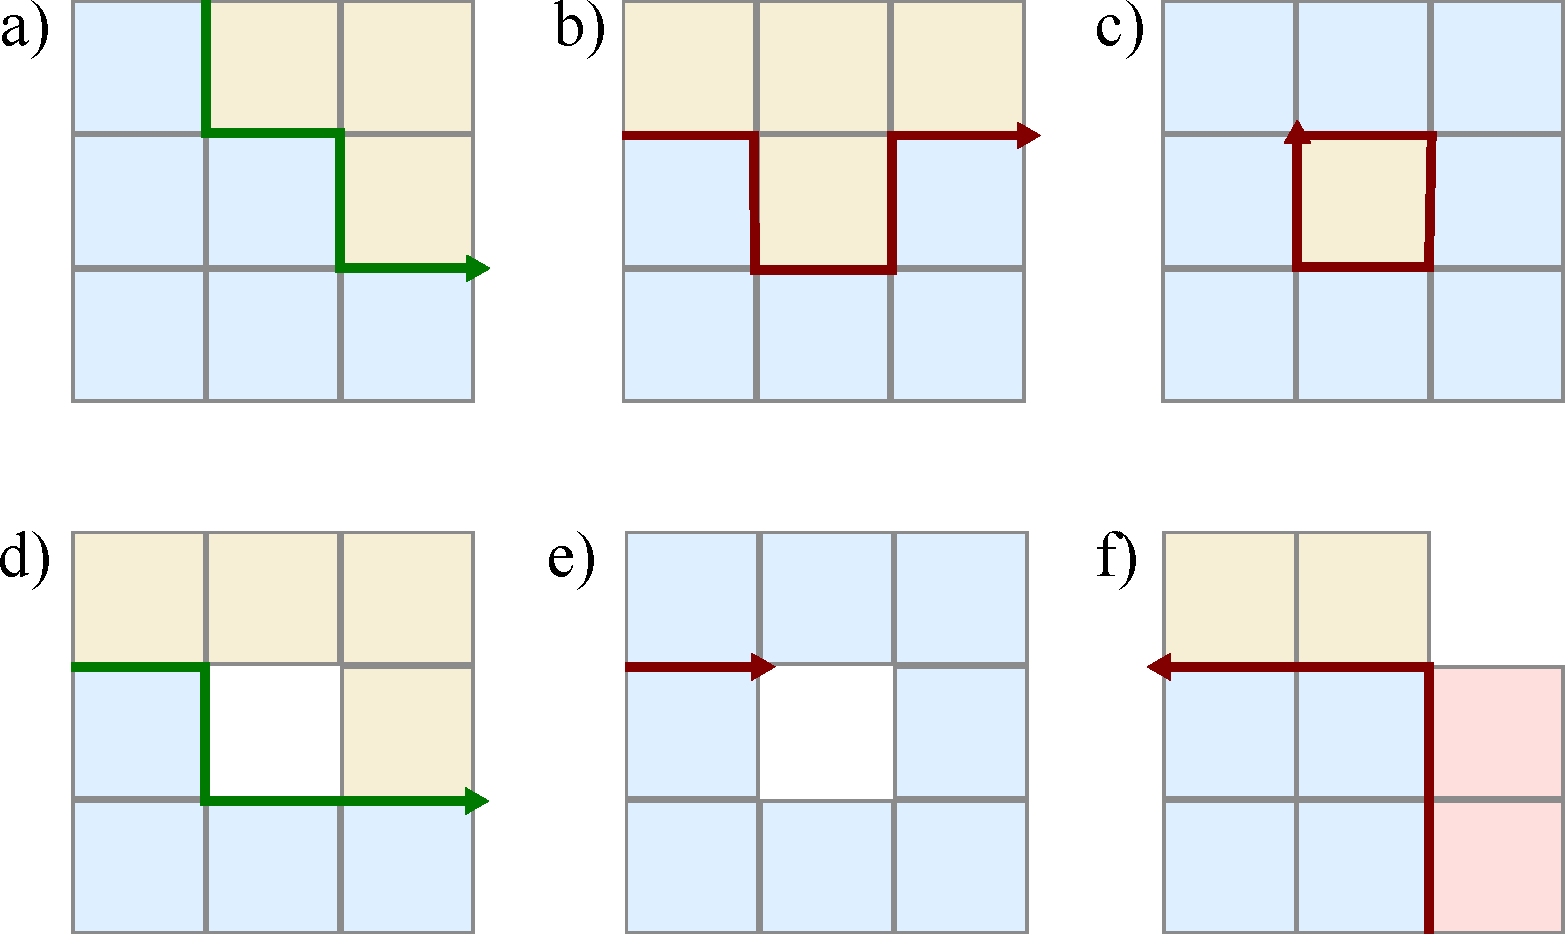
\includegraphics[width=0.6\textwidth]{figures/twocuts.pdf}
	\caption[Different cuts for polyomino shapes]{Examples for cutting polyomino shapes. The top row shows three two-cuts for a $3\times3$ shape, of which only the left one is monotone and therefor valid. The middle one creates a cave and the right one a hole. The bottom row shows cuts that do not split the polyomino into two pieces. The right one creates three sub-polyominoes and the left one does not break the polyomino at all.}
	\label{fig:twocuts}
\end{figure}
%TODO make red line dashed

\section{Two-Cutting Polyominoes}
\label{sec:twocutting}

Schmidt et al. \cite{Schmidt2018} made use of straight-line two-cuts, to handle the construction of a polyomino with more than trivial sub-assemblies.

We define a two-cut as a continues path of connections through a polyomino, that divides the polyomino into two sub-polyominoes, when these connections would be removed.
For later use in \autoref{sec:tcsa} we want to enumerate all two-cuts of a polyomino that are useful for planning.
We do not limit the cuts by only allowing straight paths like \cite{Schmidt2018}, instead we only consider monotone two-cuts.

Monotone means, that whenever the path goes into a direction it can never go into the opposite direction again.
\autoref{fig:twocuts} top-left shows a monotone two-cut through a $3\times3$ polyomino shape.
The cut starts at the top of the shape and only moves down and right.s
By removing all the connections on the path, the polyomino shape is split into two pieces.
Considering non-monotone two-cuts would create sub-assemblies with caves or holes, which could no be reassembled with our local planner.
This is the reason why they are omitted on a global scale in advance.
\autoref{fig:twocuts} top-middle shows a non-monotone two-cut creating a cave and \autoref{fig:twocuts} top-right one creating a hole.

To calculate all two-cuts of a polyomino, we take all possible monotone paths from each connection as a starting point.
A path ends when it breaks out of the polyomino or into a hole.
After the path ended its connections are removed from the polyomino and the path is added as a two-cut, if the polyomino got split into exactly two pieces.
The bottom row of \autoref{fig:twocuts} shows cuts that split the polyomino in less or more than two pieces.

% 32 possibilities for 3x3

\begin{figure}
	\centering
	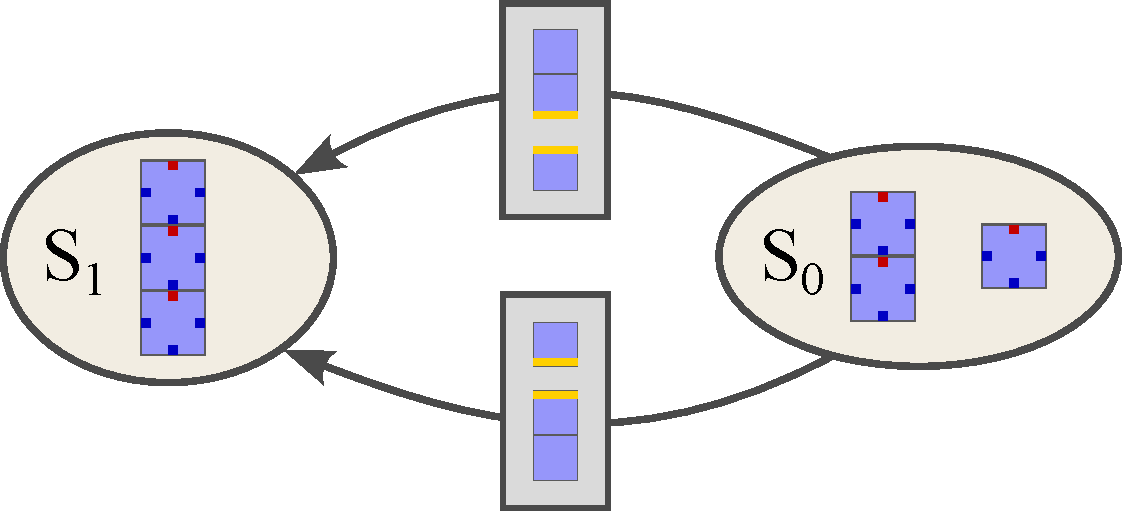
\includegraphics[width=0.45\textwidth]{figures/tcsa_multiedge.pdf}
	\caption[Two TCSA nodes connected with multiple edges.]{Two TCSA edges connecting the polyomino sets $S_0$ and $S_1$. The weights of the edges differ, since there are two ways to connect the $2\times1$ with the $1\times1$ to create a $3\times1$ polyomino. The connections are illustrated in rectangular boxes places on the edges.}
	\label{fig:tcsa_multiedge}
\end{figure}

\begin{figure}
	\centering
	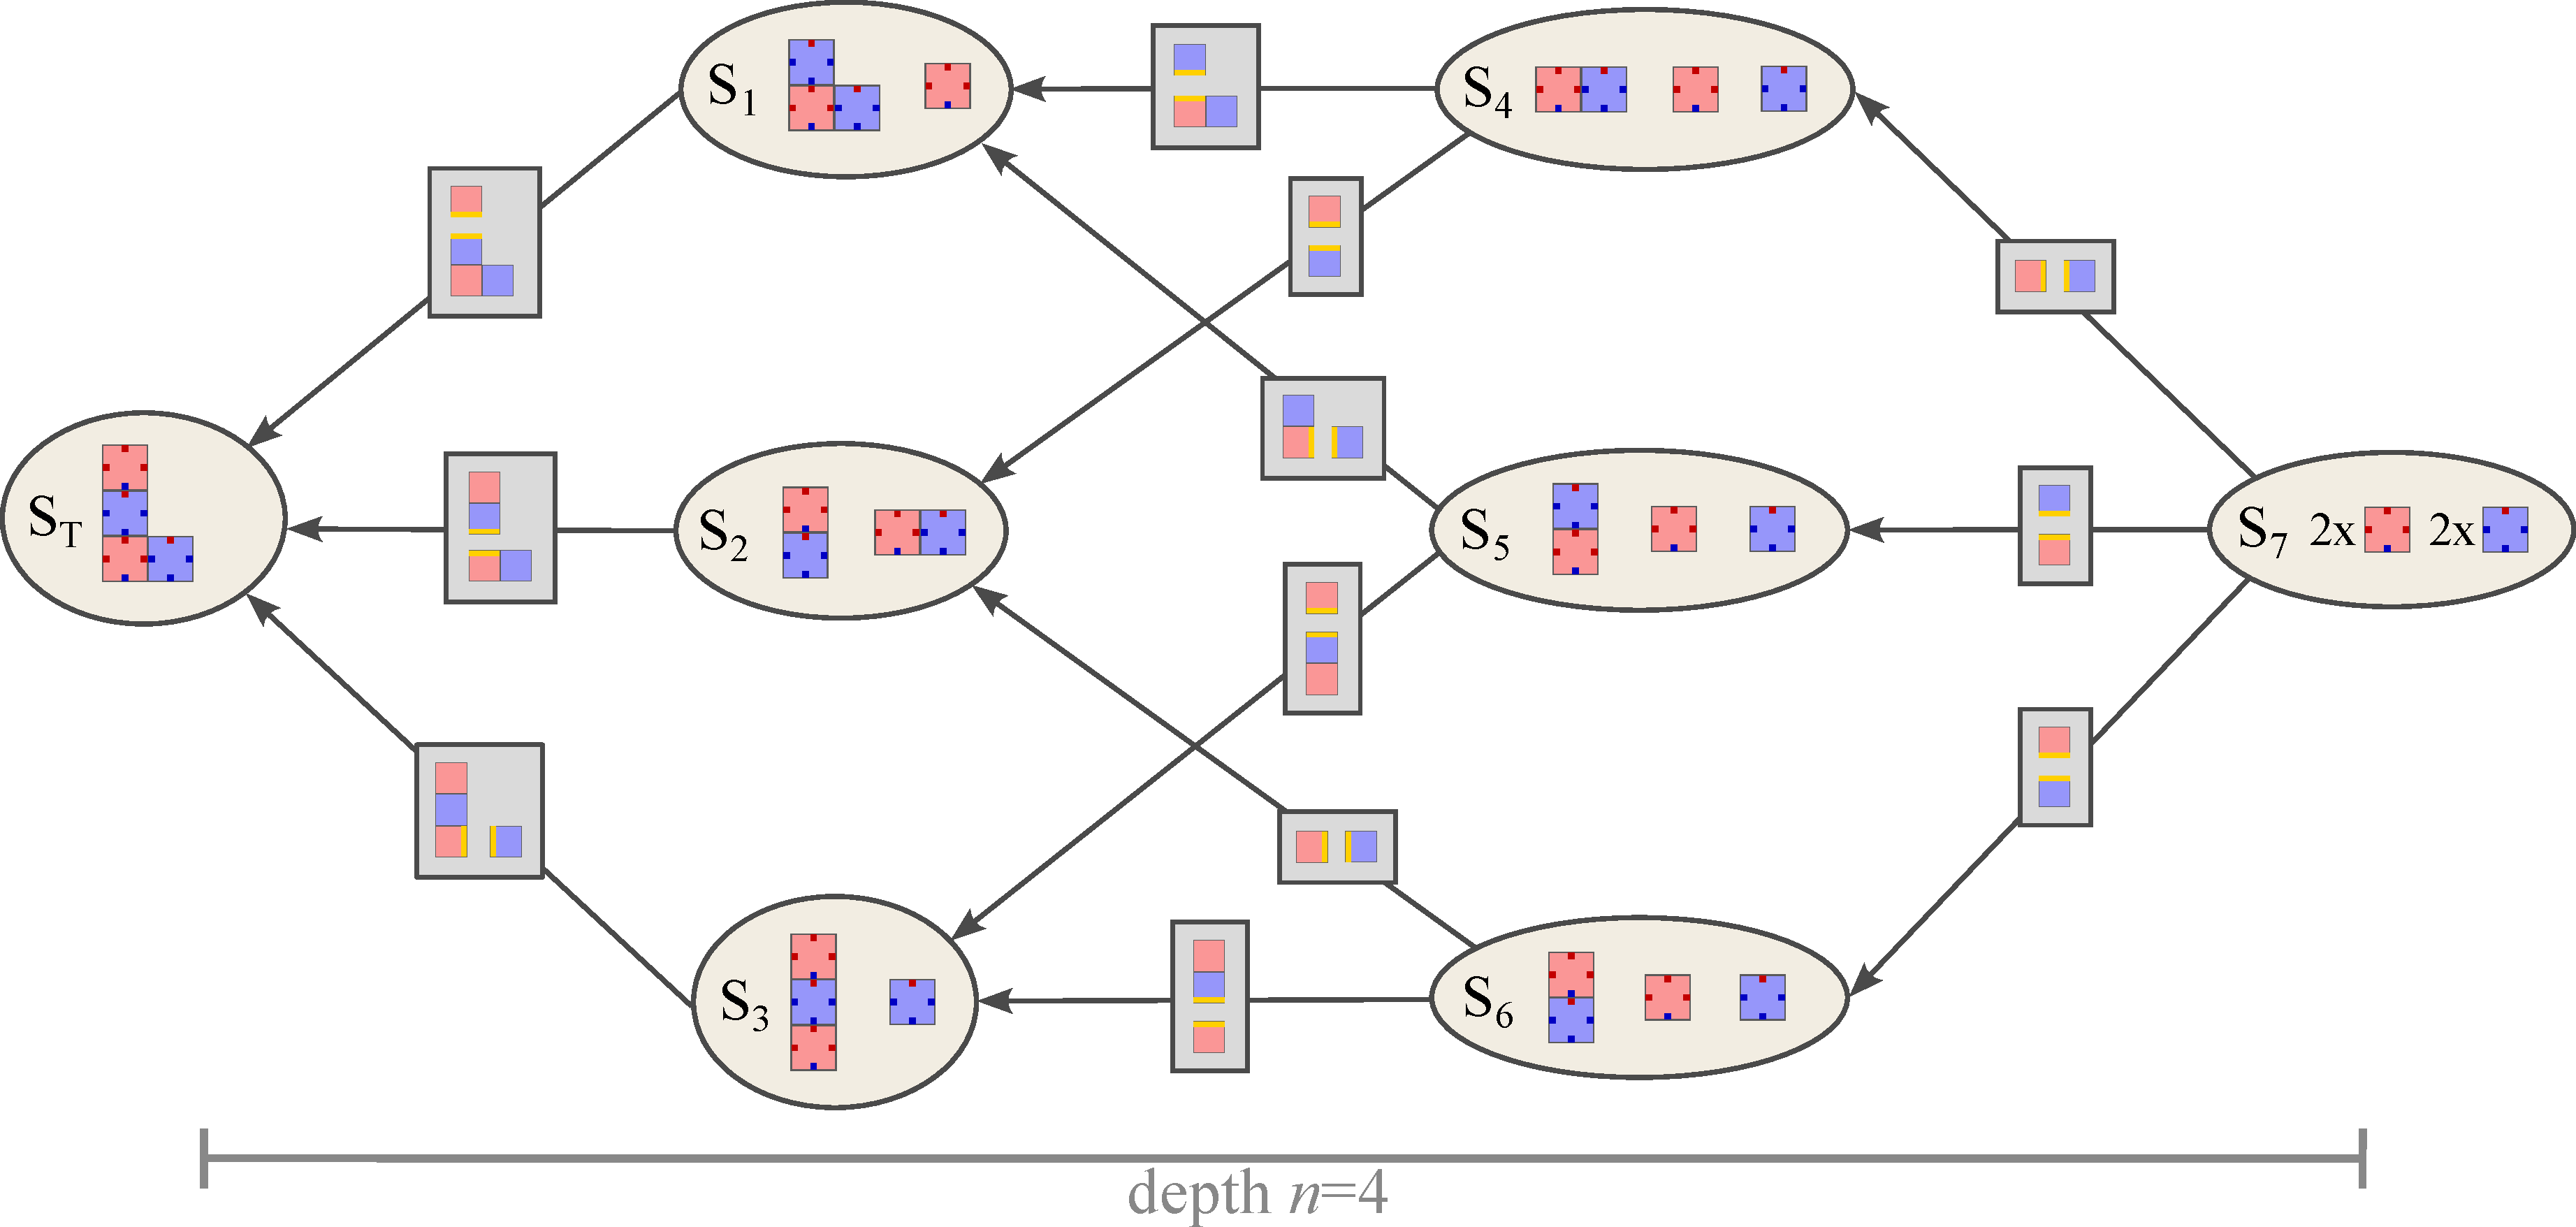
\includegraphics[width=1\textwidth]{figures/tcsa.pdf}
	\caption[Example for a two-cut-sub-assembly graph.]{Example of an TCAS graph for a four-cube L-shape. The polyomino sets are illustrated as ellipses. If the polyominoes of a set are not numbered, there is only one occurrence of this polyomino. Otherwise the number of occurrences is placed left of the polyomino. The sets are numbered, as if the graph was produces by \autoref{algo:build_tcsa}. The weight of edges are illustrated as rectangular boxes containing the polyominoes that need to be connected at specific edges, marked in yellow.}
	\label{fig:tcsa}
\end{figure}

\section{Two-Cut-Sub-Assembly Graph}
\label{sec:tcsa}

The two-cut-sub-assembly graph, short TCSA graph, functions as a building instruction for a specific target polyomino, we will call it $G_{TCSA}(T)$.
The TCSA graph works with sets of polyominoes as nodes.
While a configuration $g$ holds information about orientation and position of physically distinct polyominoes, the corresponding polyomino set $S(g)$ only enumerates the polyomino types preset in $g$.
If $g$ contain multiple polyominoes of the same type, $S(g)$ still stores the amount of the polyomino type, but does not distinguish between the actual polyominoes.

Two nodes $S_0$ and $S_1$ of the TSCA graph are connected with and edge $(S_0,w,S_1)$, if $S_0$ can be transformed to $S_1$ by connecting two polyominoes contained in $S_0$.
The cube and edge information of the connections are stored as the weight $w$.
$S_0$ and $S_1$ can be connected by multiple edges, if there are different connections that produce the same outcome.
The edges differ in their weights as shown in \autoref{fig:tcsa_multiedge}.
The direction of $(S_0,w,S_1)$ always goes from $S_0$ to $S_1$, but we can reverse the definition for an edge as following:

Two nodes $S_0$ and $S_1$ are connected, if one polyomino contained in $S_1$ can be two-cut, so that the resulting polyomino set equals $S_0$.
This already provides a perspective on the use of two-cuts and the way $G_{TCSA}(T)$ is build starting with $T$.
We will further explain the building process along with an example of a TCSA graph provided in \autoref{fig:tcsa}.


\begin{algorithm}
	\caption{\scshape Build-TCSA-Graph}
	\label{algo:build_tcsa}
	\begin{algorithmic}[1]
		\REQUIRE $T$
		\ENSURE $G_{TCSA}(T)$ \COMMENT{the graph is represented by nodes $V$ and edges $E$} 
		\STATE $V \gets \{\}$
		\STATE $E \gets \{\}$
		\STATE $i \gets 0$
		\STATE $V[i] \gets S_T$	\COMMENT{$S_T$ only contains $T$}
		\WHILE[work through nodes in BFS manner]{$i < \text{\scshape Size}(V)$}
			\STATE $S_i \gets V[i]$
			\FOR[go through all polyomino types in $S_i$]{$\forall P \in S_i$}
				\FOR{$\forall tc \in \text{\scshape Two-Cuts}(P)$}
					\STATE $P_1$,$P_2 \gets \text{\scshape Cut-Polyomino}(P, tc)$
					\STATE $S_{new} \gets S_i \setminus \{P\} \cup \{P_1, P_2\}$ \COMMENT{create $S_{new}$ by removing $P$ and adding $P_1$,$P_2$}
					\IF{$S_{new} \notin V$}
						\STATE $V \gets \text{\scshape Append}(V, S_{new})$
					\ENDIF
					\STATE $E \gets \text{\scshape Append}(E, (S_{new}, tc, S_i))$
				\ENDFOR
			\ENDFOR
			\STATE $i \gets i+1$
		\ENDWHILE
		\RETURN $(V,E)$
	\end{algorithmic}
\end{algorithm}


\paragraph{Building TCSA Graph}

\autoref{algo:build_tcsa} describes the process of building $G_{TCSA}(T)$ for the target $T$.
The algorithm works through each newly added node in $V$ in a breadth-first-search manner.
The first node added to $V$ is $S_T$, which is a polyomino set only containing the target shape.

New nodes and edges are determined, by two-cutting every polyomino type $P$ in the current set $S_i$ by every possible monotone two-cut of $P$.
This is done by enumerating the two-cuts with {\scshape Two-Cuts}, the way it was described in \autoref{sec:twocutting}, and cutting $P$ at the two-cut with {\scshape Cut-Polyomino}.
The cutting results in the two sub-polyomino $P_1$ and $P_2$.
$S_{new}$ contains the same polyominoes as $S_i$ with the exception, that one occurrences of $P$ got removed and replaced by one occurrence of each $P_1$ and $P_2$.
Each $S_{new}$ is the result of cutting one polyomino of $S_i$ at a specific two-cut $tc$.
If $S_{new}$ is not already contained in $V$, we can add it to $V$ for future iterations of the breadth-first-search.

No matter if $S_{new}$ is contained in $V$ or not, an edge going from $S_{new}$ to $S_i$ with $tc$ as the weight is added to the graph edges $E$.
This allow multiple edges, as seen in \autoref{fig:tcsa_multiedge}, and multiple out going edges to different nodes, which can be observed in \autoref{fig:tcsa}, where different connections in $S_4$ lead to either $S_1$ or $S_2$.

Each two-cut applied to a polyomino set reduces its amount of polyominoes by one.
Let $n$ be the size of $T$, then $n-1$ two-cuts applied to $S_T$ will produce a polyomino set $S_{trivial}$ containing only trivial polyominoes, as it is the case for $S_7$ in \autoref{fig:tcsa}.
All $S_i$ will inevitably end up in this situation and the algorithm will return $(E,V)$, since trivial polyominoes can not be cut anymore.
This means that no matter which connections are chosen along the way, $n-1$ edges will always be needed to get from $S_{trivial}$ to $S_T$.
We describe this attribute, by giving the TCSA graph a depth of $n$.
The depth is also illustrated in \autoref{fig:tcsa} and the numbering of the nodes matches the way they got added by \autoref{algo:build_tcsa}.

\begin{figure}
	\centering
	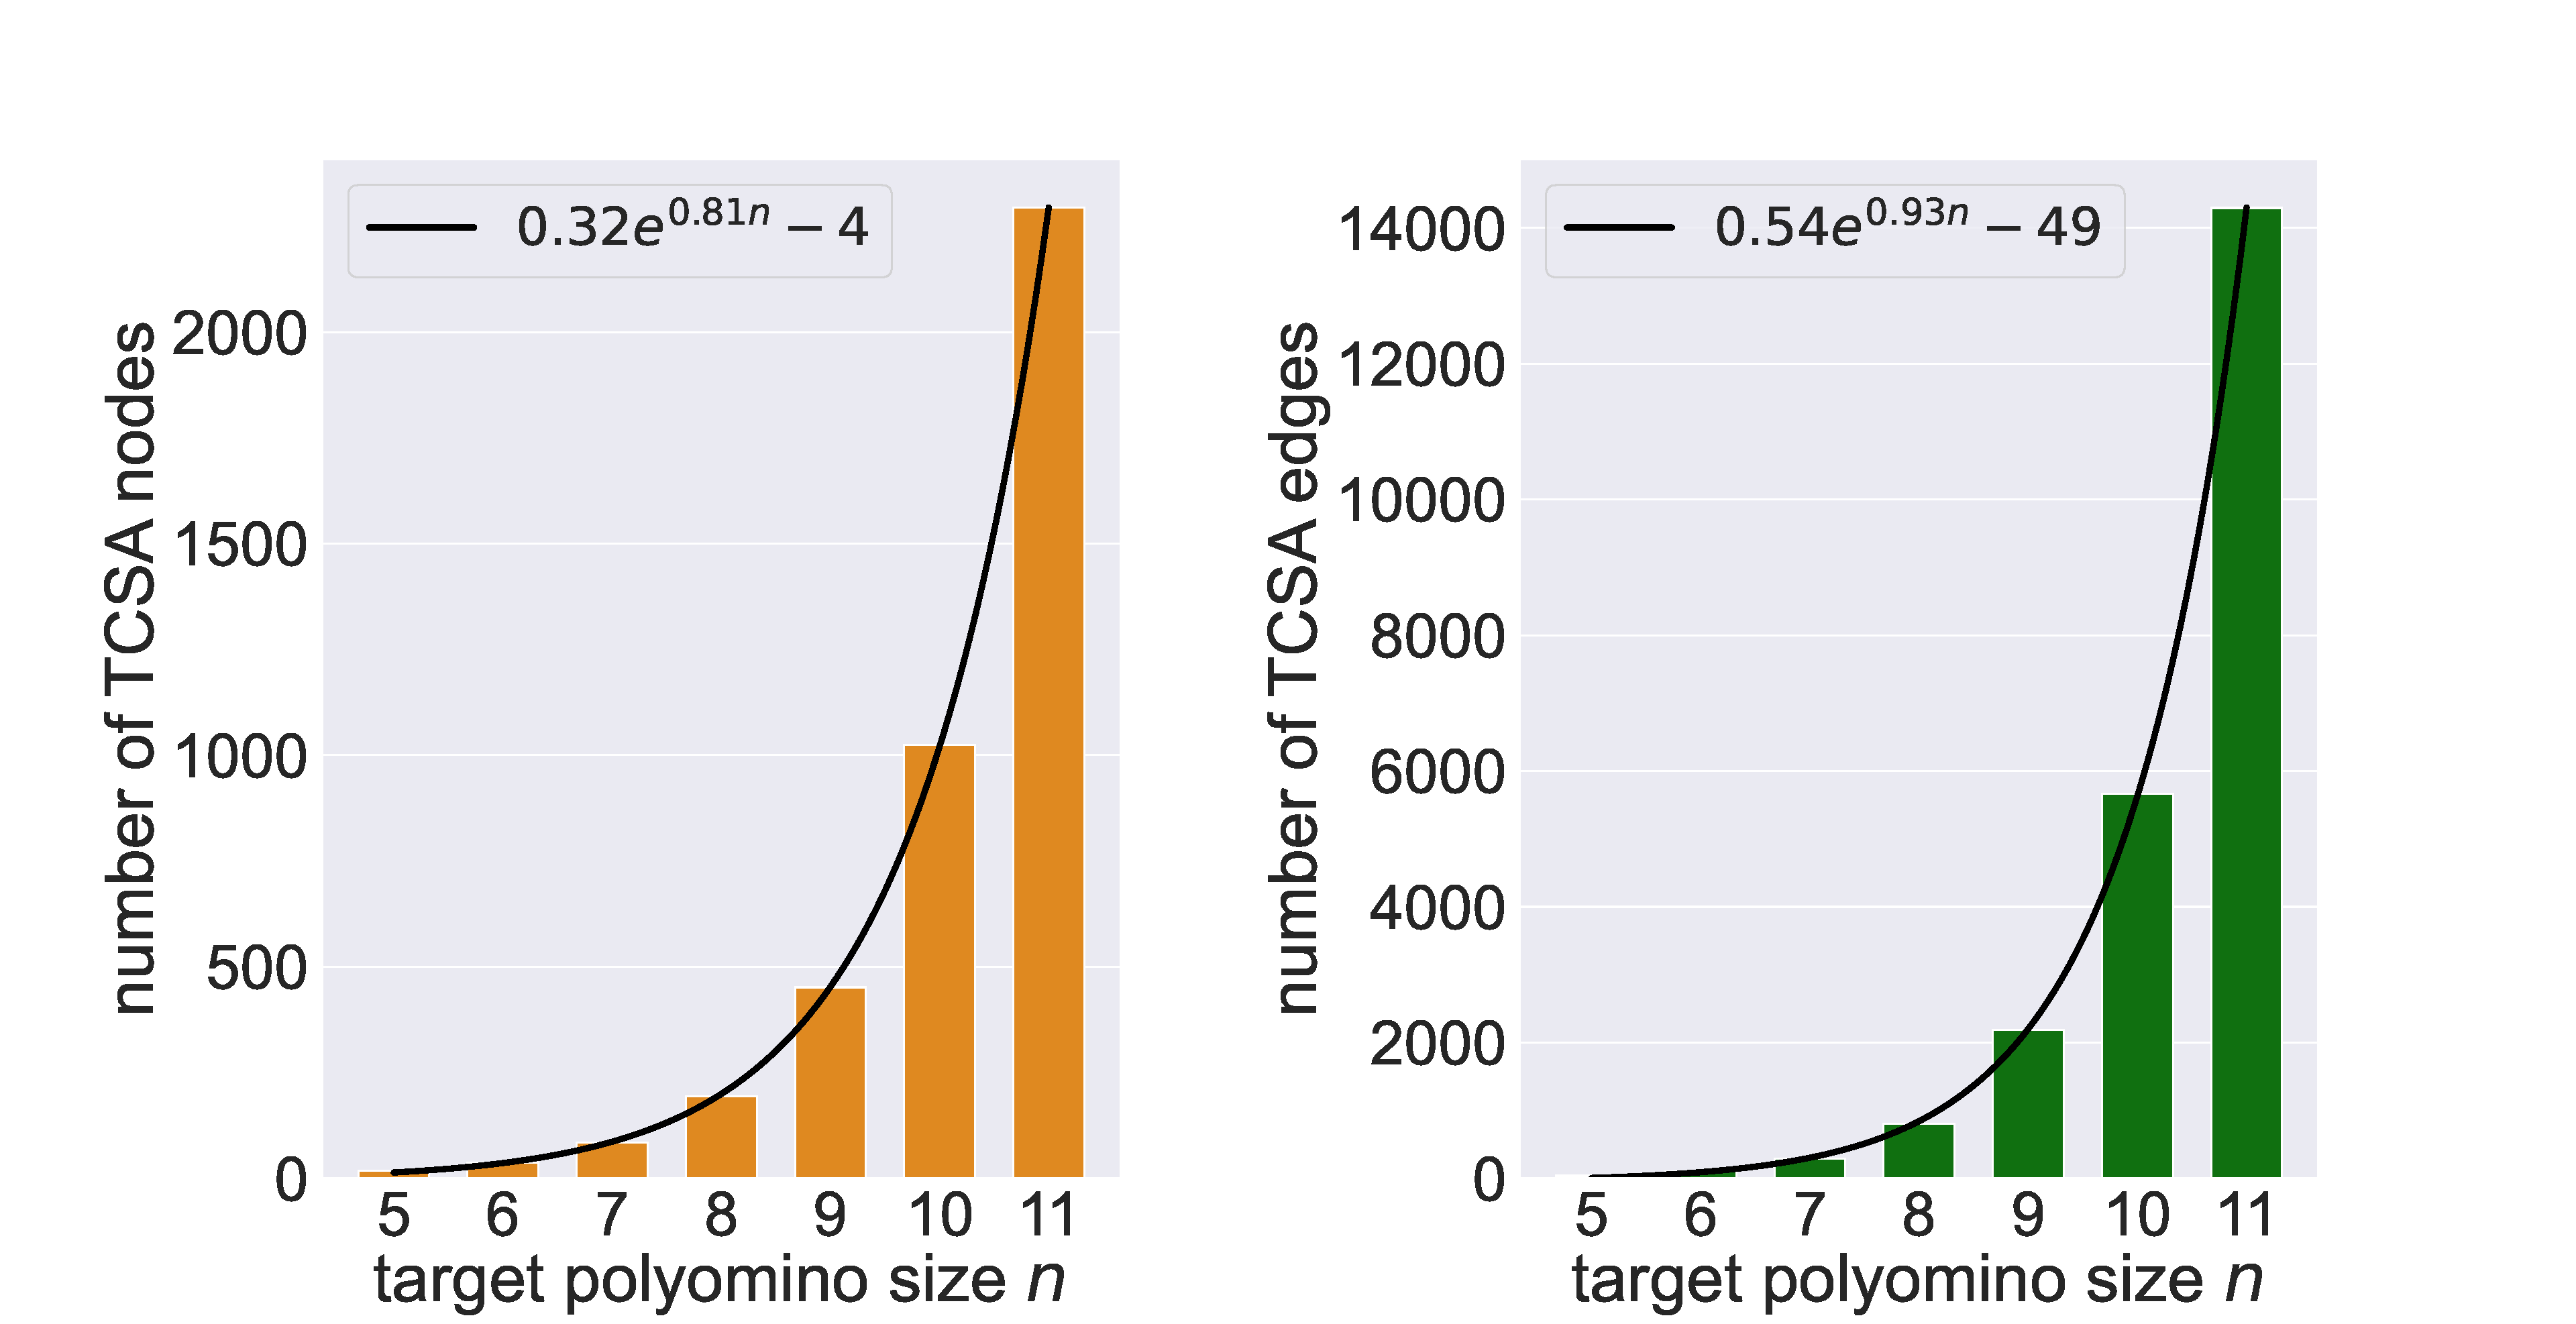
\includegraphics[width=0.80\textwidth]{figures/plots/tcsa_nodes_edges.pdf}
	\caption[Average TCSA nodes and edges for target size $n$.]{Average number of nodes (left) and edges (right) of a TCSA graph for different target sizes $n$.
	For each target size $200$ samples of randomly generated polyominoes were taken.}
	\label{fig:tcsa_plot}
\end{figure}

\subsection{Complexity}

% sterling numbers second kind as upper bound: find literatur
% connectivity cuts notes, monotonie cuts notes
% Access to graph in O(1) due to hash comparing.
% Creation complex but worth it -> minimize sim-time
% show practical data for tcsa-notes per size. Box-Whisker PLOT


\begin{figure}
	\centering
	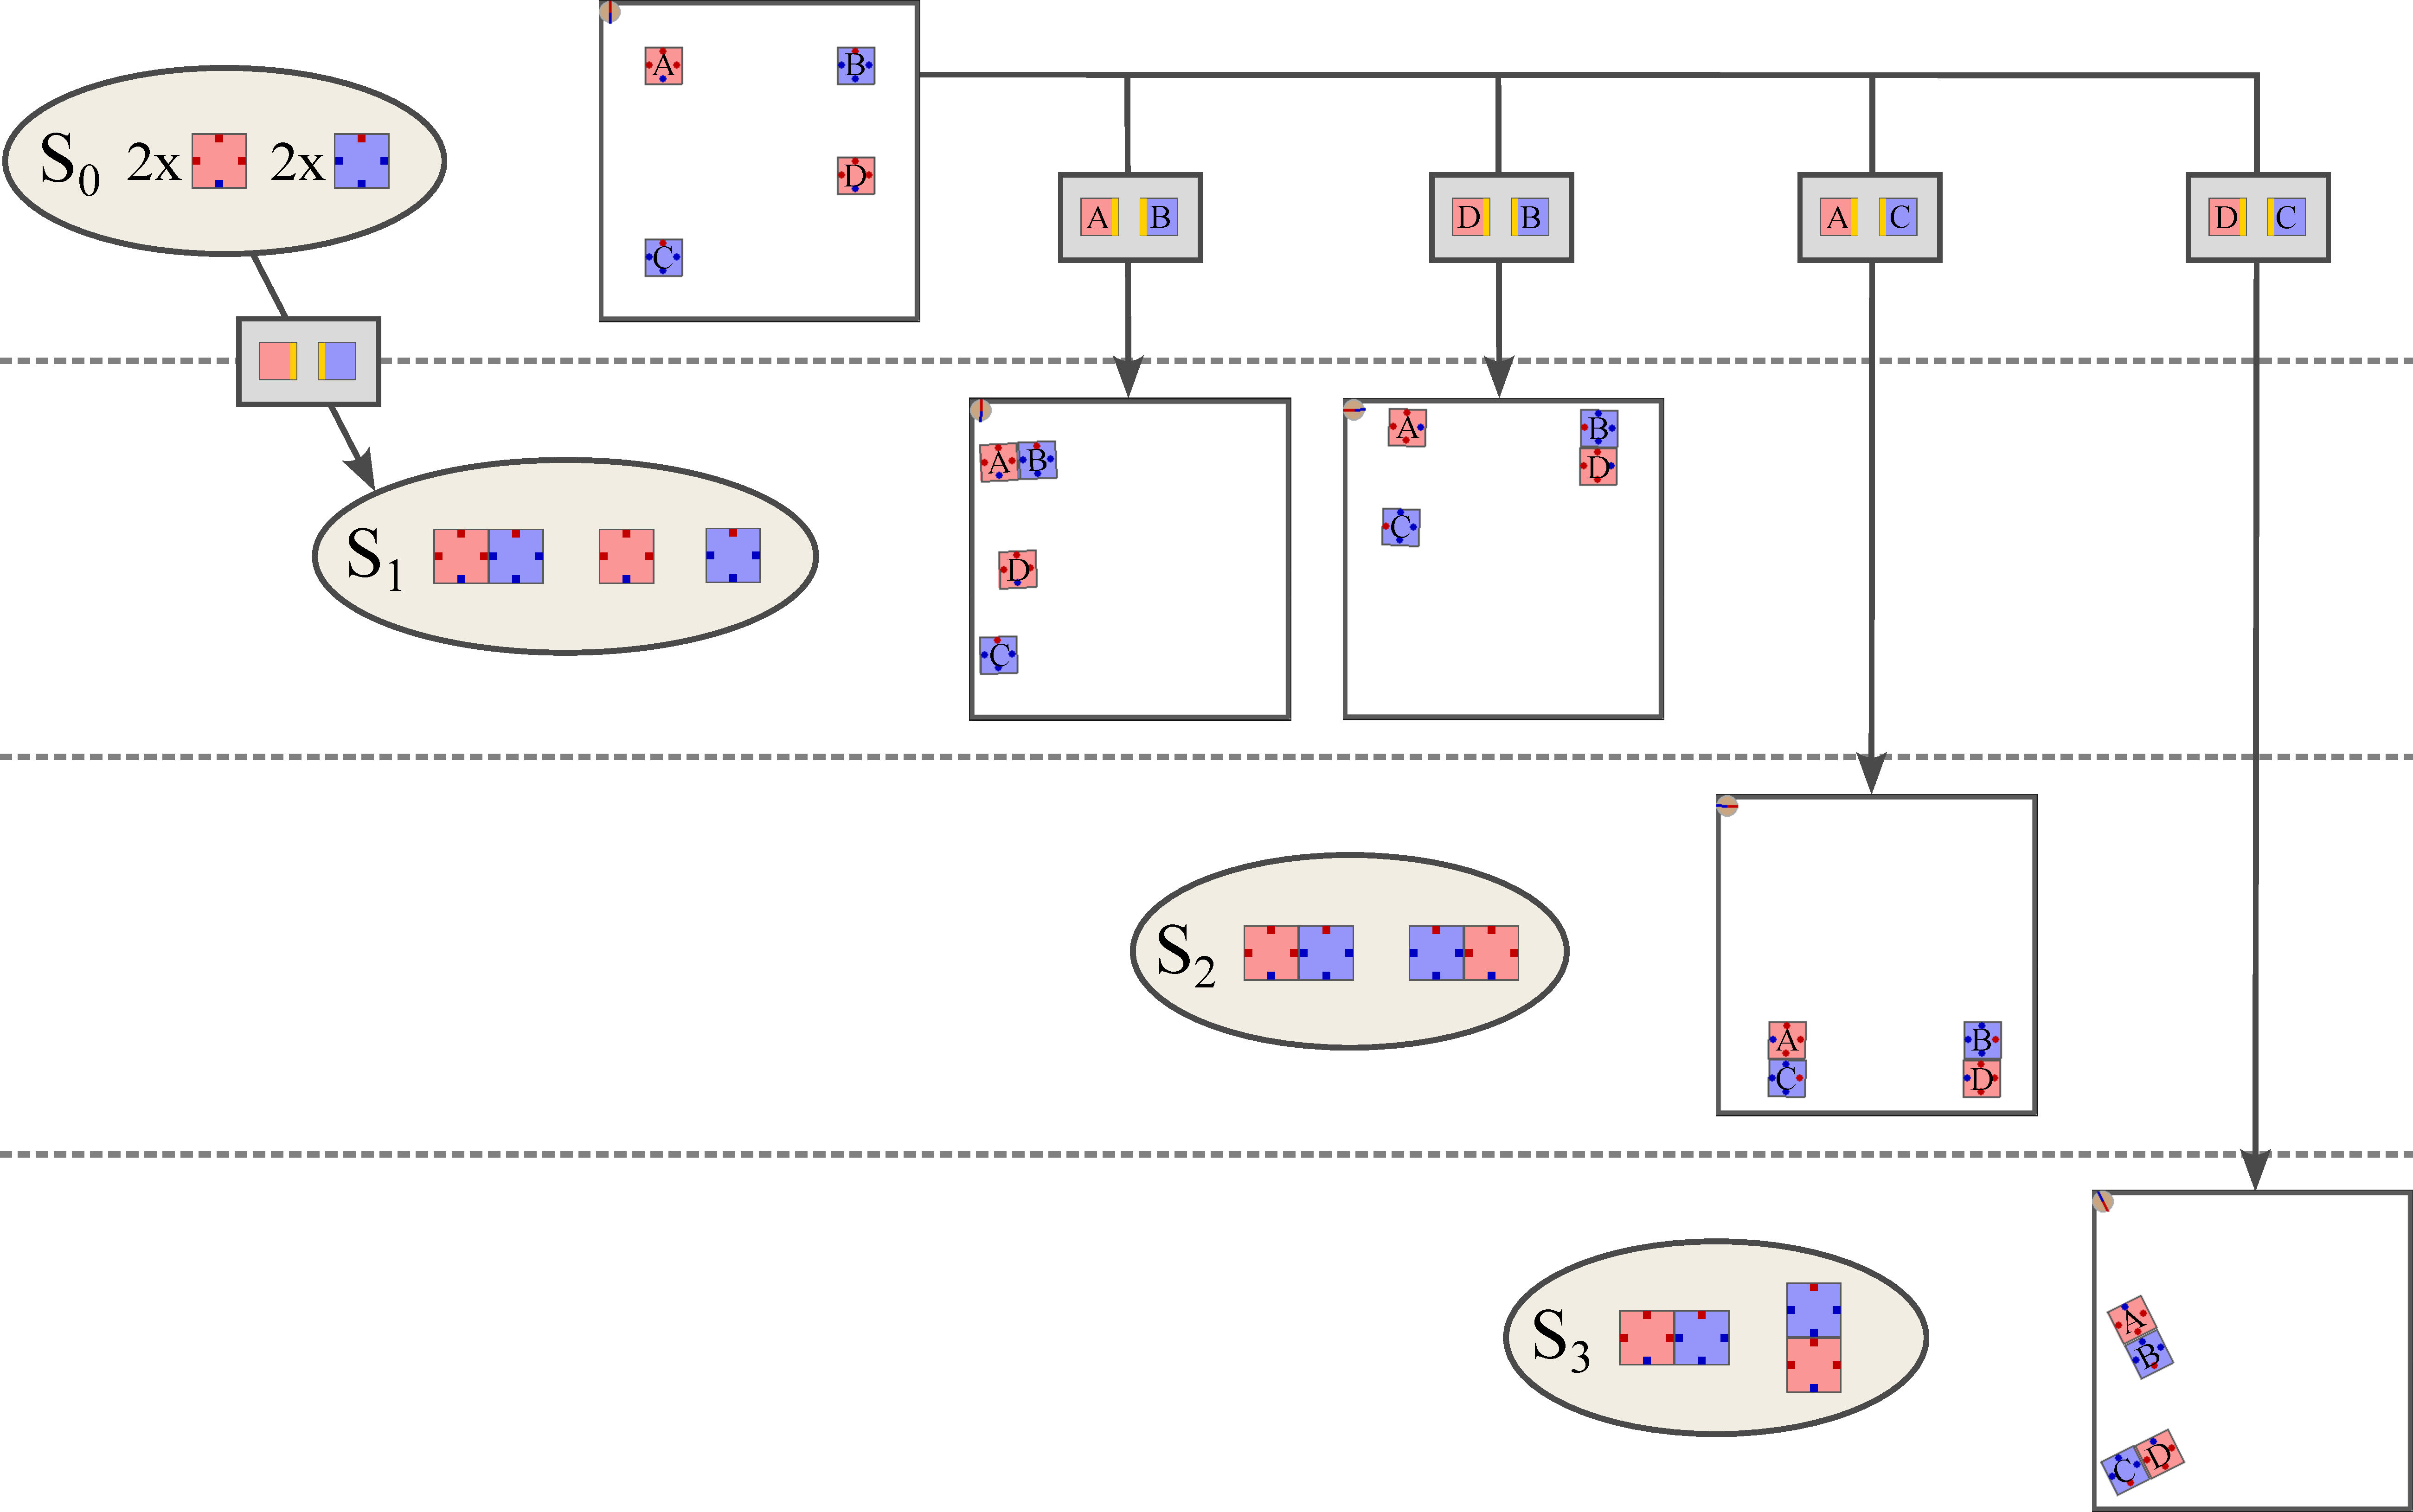
\includegraphics[width=1\textwidth]{figures/connect_options.pdf}
	\caption[Example of connection options for one TCSA edge]{All connection options when connecting a red cube at the west of a blue cube to get from $S_7$ to $S_4$. Developing a local plan for different polyomino pairs, leads to different goal configurations. $(A_1,B_1)$ and $(A_2,B_1)$ lead to the desired polyomino set $S_4$, but $(A_2,B_2)$ leads directly to $S_2$. All these sets can be found in the TCSA graph of \autoref{fig:tcsa}. The goal configuration of $(A_1, B_2)$ holds the set $S_x$, which can not be found in \autoref{fig:tcsa}. For further global planning this set could not be used.}
	\label{fig:connect_options}
\end{figure}


\section{Connection Options}
\label{sec:connect_options}

In each configuration $g$, which the global planner encounters, $G_{TCSA}(T)$ will be used to determine the next connection, that the local planner should try to establish.
For that the polyomino set $S(g)$, will be considered as a node in $G_{TCSA}(T)$.
If $S(g) \notin G_{TCSA}(T)$, $g$ can not be used to assemble $T$.
With the exception of $S_T$ all nodes have out-going edges in a TCSA graph.
All out-going edges of $S(g)$ provided connections for the local planner, that bring the global planner closer to assembling $T$.

For instance, if $S(g) = S_7$ in \autoref{fig:tcsa}, three out-going edges provide three connections to choose from, but that is not all.
Lets assume the global planner decides to connect a red cube at the west edge of a blue cube to end up in a configuration $g_2$ with $S(g_2) = S_4$.
Since $S_7$ contains multiple polyominoes for the same type, there is more than one way to achieve this.
\autoref{fig:connect_options} illustrated all the different connection options for this example case.
You can also see how theses options differ in the goal configurations the local planner ended in.

Let $L_A$ and $L_B$ be collections of the physically distinct polyominoes for the polyomino types $A$ and $B$.
When $A$ and $B$ are about to be connected as the weight of a TCSA edge dictates, there are $\left| L_A \times L_B \right|$ polyomino pairs to choose from.
If $A = B$, the options where a polyomino will be connected with itself can be eliminated.

With multiple edges and various polyomino pairs per edge, many options emerge for the global planner to consider.
We examined three sorting strategies for these options, to provide an order of best probable outcome, the global planner can work through. 

\paragraph{Minimal Distance}

The minimal distance sorting sorts connection options based on the distance between the cubes that are about to be connected.
The idea is that a smaller distances requires less movement to connect, which means shorter simulation time and lower plan costs of the resulting plan.
Due to sliding on walls and different pivot walking distances, this is not true in every case, but it remains a good heuristic for sorting.
Less movement might even prevent unwanted sub-assemblies.

\paragraph{Grow Largest Component}

Another approach is to grow the largest component.
The options are sorted into classes of maximum polyomino sizes in the resulting polyomino sets.
We prefer TCSA edges that lead to sets containing the biggest polyominoes.
When the options for $S_4$ in \autoref{fig:tcsa} are sorted, the one leading to $S_1$ is preferred over the one leading to $S_2$, because $S_1$ contains a polyomino of size $3$, while $S_2$ only contains polyominoes of size $2$. 
The options within each class are sorted with the minimal distance approach.

If no other sub-assemblies occur, growing the largest component behaves like one-tile-at-a-time assembly.
The benefit is, that even if they occur the TSCA graph can provide solutions to integrate them if possible.
Larger polyominoes generally move faster acting positive on plan costs.

\paragraph{Grow Smallest Component}

Oppositely to growing the largest component, options can be sorted by the smallest maximum size of polyominoes in polyomino sets.
This avoids working with large polyominoes, which are faster, but also need more simulation time to perform rotations and can be hard to handle, because of sheer size.
It wil be interesting to see how these complementary methods perform.


\section{Use of Local Planner}
\label{sec:local_in_global}

The local planner develops plans for connections chosen from the different connection options presented in \autoref{sec:connect_options}.
For the local planner only one connection, out of the path of connections stored in the weight of a TSCA edge, needs to be picked.
Whenever a path consists of both north-south and east-west connections, a north-south connection is preferred.
This is done to perform offset-aligning instead of straight-aligning (\autoref{sec:align}), for an easier slide-in.
Besides of that, the choice of connection is irrelevant, since all connections in the path lead to the same outcome.

When the local planner successfully connects the desired polyominoes, other sub-assemblies can lead to a different polyomino set than expected.
This is not necessarily bad, as long as the resulting set is contained in $G_{TCSA}(T)$.
In-fact, more sub-assemblies decrease the number of polyominoes in the workspace, which brings the goal of assembling $T$ even closer.
Layers of depth were skipped in the TCSA graph, so that it might be possible to assemble $T$ with less than $n-1$ local plans.
This can be seen in \autoref{fig:connect_options}, where $A_2$ and $B_2$ were connected. 
The resulting polyomino set matches with $S_2$ instead of $S_4$ of the nodes from \autoref{fig:tcsa}.

Like already mentioned in \autoref{sec:connect_options}, when the resulting polyomino set is not in $G_{TCSA}(T)$, it is not possible to assemble the target from that configuration.
This can be seen in \autoref{fig:connect_options}, when connecting $A_1$ and $B_2$.
For global use we add a new failure condition to the local planner, which checks if the polyomino set of the configuration in the workspace is contained in $G_{TCSA}(T)$.
If not, the planner immediately states failure and avoids spending simulation time on a configuration with no further use.

The local planner might even fail to establish the desired connection.
If the resulting polyomio set is contained in $G_{TCSA}(T)$, global planning can continue, but there are certain failure types that are not valid for further planning.
Polyomino sets with invalid polyominoes, or where connections in caves are necessary, should not be present in the TCSA graph anyway, but we also do not continue planning with a failure due to maximum movement capacity or polyominoes being stuck.




\section{Global Planning Algorithm}
\label{sec:global_algo}

% use of tcsa-graph
% limit number of cubes to target size
% check inclusion of poly set from config in tcsa-graph
% example early failure if initial is not in tcsa

% provide algorith
% DFS traversal. try to get to target as fast as possible
% Fall back if all options tried
% note that we not traverse tcsa graph we actually traverse configurations.
% When 2 configs with same polyset occure still try all options for both, because position differs

\subsection{Complexity}

% best case 1 local plan. realistic best case n-1
% we are not limited by notes in tcsa, because n configs for 1 note
% for each note there is a constant number of options and depth smaller n-1.
% we wont run infinitly, but worst case is still bad. state example each note 50 options

\subsection{Discretize Configurations}

% dont know if I wil actually implement, but talk about benefits or why not that neccessary




\section{More Cubes than Target}
\label{sec:more_cubes}

% bigger tcsa with multiple end notes
% same tcsa
% - no simple hash check. check for set inclusion
% - a poly set can be included in multiple tcsa-notes -> increasing options per config